%%%%%%%%%%%%%%%%%%%%%%%%%%%%%%%%%%%%%%%%%
% Structured General Purpose Assignment
% LaTeX Template
%
% This template has been downloaded from:
% http://www.latextemplates.com
%
% Original author:
% Ted Pavlic (http://www.tedpavlic.com)
%
% Note:
% The \lipsum[#] commands throughout this template generate dummy text
% to fill the template out. These commands should all be removed when 
% writing assignment content.mus
%
%%%%%%%%%%%%%%%%%%%%%%%%%%%%%%%%%%%%%%%%%

%----------------------------------------------------------------------------------------
%	PACKAGES AND OTHER DOCUMENT CONFIGURATIONS
%----------------------------------------------------------------------------------------

\documentclass{article}

%\usepackage[brazilian]{babel}
\usepackage[utf8]{inputenc}
\usepackage{fancyhdr} % Required for custom headers
\usepackage{lastpage} % Required to determine the last page for the footer
\usepackage{extramarks} % Required for headers and footers
\usepackage{graphicx} % Required to insert images
\usepackage{float}
\usepackage{listings}
\usepackage{amsmath}
\usepackage[colorlinks=true, pdfborder={0 0 0}, urlcolor=blue, linkcolor=black]{hyperref}

\graphicspath{ {img/} }

% Margins
\topmargin=-0.45in
\evensidemargin=0in
\oddsidemargin=0in
\textwidth=6.5in
\textheight=9.0in
\headsep=0.25in 

\linespread{1.1} % Line spacing

% Set up the header and footer
\pagestyle{fancy}
\lhead{\hmwkAuthorName} % Top left header
%\chead{\hmwkClass\ (\hmwkClassInstructor\ \hmwkClassTime): \hmwkTitle} % Top center header
\rhead{\hmwkClass: \hmwkTitle} % Top center header
%\rhead{\firstxmark} % Top right header
\lfoot{\lastxmark} % Bottom left footer
\cfoot{} % Bottom center footer
\rfoot{Página\ \thepage\ de\ \pageref{LastPage}} % Bottom right footer
\renewcommand\headrulewidth{0.4pt} % Size of the header rule
\renewcommand\footrulewidth{0.4pt} % Size of the footer rule

\setlength\parindent{0pt} % Removes all indentation from paragraphs

%----------------------------------------------------------------------------------------
%	DOCUMENT STRUCTURE COMMANDS
%	Skip this unless you know what you're doing
%----------------------------------------------------------------------------------------

% Header and footer for when a page split occurs within a problem environment
\newcommand{\enterProblemHeader}[1]{
\nobreak\extramarks{#1}{#1 continues in next page\ldots}\nobreak
\nobreak\extramarks{#1 (continuation)}{#1 continues in next page\ldots}\nobreak
}

% Header and footer for when a page split occurs between problem environments
\newcommand{\exitProblemHeader}[1]{
\nobreak\extramarks{#1 (continuation)}{#1 continues in next page\ldots}\nobreak
\nobreak\extramarks{#1}{}\nobreak
}

\setcounter{secnumdepth}{0} % Removes default section numbers
\newcounter{homeworkProblemCounter} % Creates a counter to keep track of the number of problems

\newcommand{\homeworkProblemName}{}
\newenvironment{homeworkProblem}[1][\arabic{homeworkProblemCounter}]{ % Makes a new environment called homeworkProblem which takes 1 argument (custom name) but the default is "Problem #"
\stepcounter{homeworkProblemCounter} % Increase counter for number of problems
\renewcommand{\homeworkProblemName}{#1} % Assign \homeworkProblemName the name of the problem
\section{\homeworkProblemName} % Make a section in the document with the custom problem count
\enterProblemHeader{\homeworkProblemName} % Header and footer within the environment
}{
\exitProblemHeader{\homeworkProblemName} % Header and footer after the environment
}

\newcommand{\problemAnswer}[1]{ % Defines the problem answer command with the content as the only argument
\noindent\framebox[\columnwidth][c]{\begin{minipage}{0.98\columnwidth}#1\end{minipage}} % Makes the box around the problem answer and puts the content inside
}

\newcommand{\homeworkSectionName}{}
\newenvironment{homeworkSection}[1]{ % New environment for sections within homework problems, takes 1 argument - the name of the section
\renewcommand{\homeworkSectionName}{#1} % Assign \homeworkSectionName to the name of the section from the environment argumen
\subsection{\homeworkSectionName} % Make a subsection with the custom name of the subsection
\enterProblemHeader{\homeworkProblemName\ [\homeworkSectionName]} % Header and footer within the environment
}{
\enterProblemHeader{\homeworkProblemName} % Header and footer after the environment
}
   
%----------------------------------------------------------------------------------------
%	NAME AND CLASS SECTION
%----------------------------------------------------------------------------------------

\newcommand{\hmwkTitle}{Proposal for Bachelor Thesis 01} % Assignment title
\newcommand{\hmwkDueDate}{26 October 2014} % Due date
\newcommand{\hmwkClass}{} % Course/class
\newcommand{\hmwkClassFull}{} % Course/class
\newcommand{\hmwkClassTime}{} % Class/lecture time
\newcommand{\hmwkClassInstructor}{} % Teacher/lecturer
\newcommand{\hmwkAuthorName}{William Bombardelli da Silva} % Your name

%----------------------------------------------------------------------------------------
%	TITLE PAGE
%----------------------------------------------------------------------------------------

\title{
%\vspace{2in}
\Large\textmd{\textbf{\hmwkClassFull}}\\
\normalsize{\textbf{\hmwkTitle}}\\
\normalsize\vspace{0.1in}\small{\hmwkDueDate}\\
%\vspace{0.1in}
\large{\textit{\hmwkClassInstructor\ \hmwkClassTime}}
%\vspace{3in}
}

\author{\textbf{\hmwkAuthorName}}
\date{} % Insert date here if you want it to appear below your name

%----------------------------------------------------------------------------------------

\begin{document}

%\maketitle
{\centering
\Large\textmd{\textbf{\hmwkClassFull}}\\
\normalsize{\textbf{\hmwkTitle}}\\
\normalsize\vspace{0.1in}\small{\hmwkDueDate}\\
%\vspace{0.1in}
\large\textbf{\hmwkAuthorName}
%\large{\textit{\hmwkClassInstructor\ \hmwkClassTime}}\\

}
%----------------------------------------------------------------------------------------
%	TABLE OF CONTENTS
%----------------------------------------------------------------------------------------

%\setcounter{tocdepth}{1} % Uncomment this line if you don't want subsections listed in the ToC

%\newpage
%\tableofcontents
%\newpage

% To have just one problem per page, simply put a \clearpage after each problem

\begin{homeworkProblem}[Beyond the UML2Java: Defining a Network of Models]
	\begin{section}{Introduction}
	This document intents to describe the proposal number 01 for bachelor thesis by William Bombardelli da Silva, student of Informatik Bachelor in the Technische Universität Berlin, student number 364927.
	
	The goal of this bachelor thesis is to report the current state of research and to develop new contributions both theoretical and practical. By being so, the thesis aims to investigate a problem of software model synchronization in the context of Model-driven Engineering. More specifically the problem of building a network of software meta-models describing the relations (or transformations) between them is to be tackled.
	\end{section}
	
	\begin{section}{Key-words}
	Model Synchronization, Iterative Model Transformation, Model Transformation, Model-driven Engineering, Software Engineering.
	\end{section}	
	
	\begin{section}{Theme Description}
	Recent techniques of software engineering have been using the concept of software models in the construction of software systems. According to [Czarnecki and Helsen 2006] "\textit{Models are system abstractions that allow developers and other stakeholders to effectively address concerns, such as answering a question about the system or effecting a change}”. By defining a model as a system abstraction, it becomes clear, that a software system might have several models abstracted from it, each one representing certain aspects of the whole system. These models also have relations between themselves, in the sense that they all are supposed to describe the actual system consistently by not presenting logical contradictions. Here examples of models are \emph{UML class diagram}, \emph{Use Cases}, or even the source-code itself.
	
	The possible diversity of models in a system and the vast number of their relationships suggests the creation of a network of models for a system. Where each component of the network is a different model, and two components are interconnected if, and only if their respective models have a relationship between them. One can see this network alternatively as a graph, whereas each vertex \emph{v} represents a model, and an edge connecting $v_i$ and $v_j$ exists if, and only if there is a relationship defined between both models \emph{i} and \emph{j}.
	
	The goal of this bachelor thesis is then to create a network of typical meta-models (M2-level models, see [QUOTE]) commonly used in software systems in current industry projects, writing down firstly the meta-model definitions, and later writing their relationships. In the end of the creation of this network it is expected the inference of theoretical properties to arise and the creation of a report comprising the difficulties and the next challenges for the problem. The meta-models used might be narrowed to MOF compliant (see [QUOTE]) meta-models though, including \emph{Java code}, \emph{UML diagrams}, \emph{formal specifications}, among others.
	%TODO: QUOTE MOF
	%TODO: QUOTE M2
	\end{section}
	
	\begin{section}{Motivation}
	The lack of relation definitions in current literature for non-common models in research, but extensively used models in industry, is the main motivation for this thesis. Examples of these models are \emph{OCL contracts} (used in design by contract methods), unit tests, textual documentation and formal specification. It means, that the success of this thesis might bring the contribution of delivering a consistent and clear definition of a network with these non-common models to both the research and industry community. Therefore the availability of such a network might finally allow the extensive use of Model-driven Engineering in the praxis $-$ bridging the gap between system abstractions and its concrete form $-$ and the further development of more sophisticated model synchronization methods.
	
	It is worth to note also, that the contribution of this thesis might help enhancing the quality of current software construction and therefore lessening the number of software problems and errors, what is an endemic problem nowadays.
	\end{section}
	
	\begin{section}{State of Current Research}
	A research road-map for model synchronization found in [France 2007] gives an overview on the realm, and an interesting point of view about the challenges. In [Mens 2006] a taxonomy for model transformation is proposed, what helps to carry more precise analysis. In [Czarnecki and Helsen 2006] a survey was driven and a framework for classification of model transformation approaches was presented.
	In [Diskin 2015] a taxonomy for a network of models is presented and in [Diskin 2011] a theoretical algebraic basis is proposed. These both works may be used extensively in our further development. Additionally, one can judge by the date of publication of these works, that the topic of building a network of models is extremely active and is actually the edge of current academic research, what motivates even more the development of this thesis.
	\end{section}
	
	\begin{section}{Concepts Definition}
	Below is a list of necessary basic concepts, that will be used throughout this document.
	
	\textbf{Model:} The definition for software model used is: “Models are system abstractions that allow developers and other stakeholders to effectively address concerns, such as answering a question about the system or effecting a change” [Czarnecki and Helsen 2006]. Examples of models, according to this definition, are \emph{UML diagrams}, \emph{OCL expressions}, \emph{relational database diagrams}, or even source-code.
	
	\textbf{Modeling Language:} For the scope considered here, modeling language is broadly defined as a language used to create models, that can be textual or graphical and may occur in several paradigms. Among them, functional, declarative or operational paradigms.
	
	\textbf{Model Relation:} Model relation here is defined abstractly as every relationship or constraint possible to happen between one source model and one target model.
	
	\textbf{Model Transformation:} Model transformation can be viewed as common data transformation – very common in computer science – with the specificity of dealing with models [Czarnecki and Helsen 2006]. In these terms, one can see model transformation from several points of view, for example as a sequence of operations/modifications over one model; or as a function, whose inputs relate to initial models and the output reflect the updated models. The borders between model transformation and model relation are sometimes fuzzy and both terms might be used interchangeably.
	
	\textbf{Model Synchronization:} The goal of model synchronization is to maintain all relations between the models of a system consistent/correct as updates are performed over them [Diskin 2011]. Model synchronization may be seen as a procedure, a series of model transformations; as a function, which output – e.g. consistent updated set of models – is determined by the inputs – e.g. consistent set of models plus transformations to be executed; or even as a relation between set of models.
	As model synchronization is a relative new field of study, no fixed definition or approach is consensus between researchers, what brings up a variety of possible strategies and conjectures to solve the problem.
	
	\textbf{Network of Models:} A network of models of a system $S$ is an undirected graph $G = (V,E)$, whereas each vertex $v_i \in V$ represents a unique model $i$ of $S$, and an edge $(v_i, v_j)$ exists if, and only if there is a relation defined between both models $i, j \in S$.
	\end{section}
	
	\begin{section}{Problem Definition}
	The problem tackled in this thesis is the problem of constructing a network of meta-models of an example system, which should be similar to the common information systems from the current state of industry.
	
	An example of a possible network is supposed to look basically like the figure \ref{fig:NetExample01}:
	\begin{figure}[H]
	\centering
	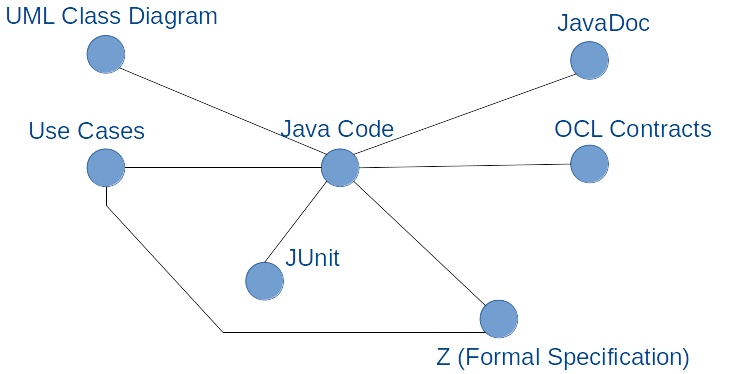
\includegraphics[scale=0.5]{NetworkExample_01}
	\caption{Example of a possible network of meta-models to be constructed. Like stated in the text, the meta-models are chosen accordingly basically to the frequency they are used currently in the software engineering industry.}
	\label{fig:NetExample01}
	\end{figure}
	
	In the first moment the meta-models comprised in the network are to be defined. So for example, in this phase the definition of the meta-model \emph{UML} or the meta-model \emph{Java Code} will be written. This can be made using the \emph{XMI} standard from \emph{OMG} [QUOTE].
	%TODO: QUOTE XMI
	Later on, given the defined meta-models (this is the vertices of the graph), their relations can be written (this is the edges of the graph). This can be made with model transformations languages like \emph{ATL}, \emph{QVT (Query/View/Transformation)} or even with \emph{Triple Graph Grammars} (see [QUOTES]). So for example, in this phase the inherent relation between the \emph{UML Class Diagram} meta-model and the \emph{Java Code} meta-model will be written. Analogously, the relations between \emph{Java Code}, \emph{JavaDoc}, \emph{JUnit} and other meta-models can be also defined. Some of these relations might be found in current research literature, others might have to be found during the development of this thesis.
	%TODO: QUOTE ATL
	%TODO: QUOTE QVT
	%TODO: QUOTE TGG
	After having this network of meta-models (M2-level models) ready, creating an actual network of models (M1-level models) of any software system is trivial, thus study cases and example networks can be developed.
	
	In the end the result might be a network of meta-models useful in the praxis, in benchmarks and further researches as well. Theoretical properties, like completeness, correction and soundness of relations, and a record of the difficulties found are expected to arise from such development.
	\end{section}
	
	\begin{section}{Possible Difficulties}
	Possible difficulties that can be found throughout the development of this thesis include:
	\begin{itemize}
		\item The definition of the meta-models in the network of meta-models might be complicated and require relatively extensive work. For example, the definition of the \emph{Java Code} meta-model can be very broad and thus a narrowing of it is likely to be necessary.
		\item Some relations of the network might be difficult or complicated to build, requiring much time, so that it is not possible to include it in the scope of this thesis.
		\item Problems like cycles in the network might also bring some difficulties.
	\end{itemize}
	\end{section}
	
	\begin{section}{Time Schedule}
	\begin{table}[h]
	\centering
	\begin{tabular}{l | l | l }
		\textbf{Duration} & \textbf{Start and End Dates} & \textbf{Activities} \\ \hline
			2 Weeks &	13/10/2015 to 26/10/2015 &	Initial research; definition of theme; finding of literature\\ \hline
			1 Weeks &	27/10/2015 to 02/11/2015 &	Detailed research; write of proposal; definition of scope\\ \hline
			2 Weeks &	03/11/2015 to 16/11/2015 &	Deepening in the theme; sketch of the development\\ \hline
			3 Weeks &	17/11/2015 to 07/12/2015 &	Analysis; design; pre-development phase; review; start of the writing\\ \hline
			5 Weeks &	08/12/2015 to 11/01/2016 &	Development; testing, validation and verification; review; writing\\ \hline
			2 Weeks &	12/01/2016 to 25/01/2016 &	Validation and verification; review; writing\\ \hline
			3 Weeks &	26/01/2016 to 15/02/2016 &	Finalization of writing; review\\ \hline
			1 Weeks &	16/02/2016 to 22/02/2016 &	Preparation of presentation\\ \hline
			1 Weeks &	23/02/2016 to 29/02/2016 &  Final review\\ \hline
	\end{tabular}
	\caption{Plan for the researching, developing and writing of the bachelor thesis. This schedule is organized in weeks, whereas each week has its respective activities planed.}
	\end{table}
	\end{section}
	
	\begin{section}{Bibliography}
	%TODO: [Czarnecki and Helsen 2006]
		Diskin, Zinovy, et al. "Towards a rational taxonomy for increasingly symmetric model synchronization." \textit{Theory and Practice of Model Transformations}. Springer International Publishing, 2014. 57-73.\\
		\\
		Diskin, Zinovy. "Model synchronization: Mappings, tiles, and categories." \textit{Generative and Transformational Techniques in Software Engineering III}. Springer Berlin Heidelberg, 2011. 92-165.\\
		\\
		Zinovy Diskin, Hamid Gholizadeh, Arif Wider, Krzysztof Czarnecki, "A Three-Dimensional Taxonomy for Bidirectional Model Synchronization", \textit{The Journal of Systems \& Software (2015)}, doi: 10.1016/j.jss.2015.06.003 \\
		\\
		France, Robert, and Bernhard Rumpe. "Model-driven development of complex software: A research roadmap." \textit{2007 Future of Software Engineering}. IEEE Computer Society, 2007.
	\end{section}
\end{homeworkProblem}

\end{document}

